HIVE web is a demo that implement a web interface for HIVE Core.

\subsection{Web UI for Browsing and Searching vocabularies}

We design and implement HIVE Web User Interface based on Rich Internet Application(RIA) model. 
In traditional web application, the user interface is only assigned for two tasks: display 
information and send the request to the designated web server, while all the data storage and application 
logic are maintained by the program in web server. The hindrance of traditional web application model 
created for user experience has two folds:  (1)Each request sent by user interface requires a page load 
hence reduce the responsiveness of the user interface. (2) The web page is a static document to present 
information rather than interactive application for user to control and manipulate. The computing power 
of personal computer is sufficient to process and render complex data logic in client browser. The RIA 
model distributes a part of computation to client side user interface, so that user can perform complex 
interaction with the interface without requesting the server. Furthermore, if user's interaction must 
request server to refresh some data, the client can selectively retrieve from the server only the 
information that needed to be changed, update its internal status, and redisplay the modified content.
Typical examples of RIA in the market nowadays are GMail, Google Document, etc.

We design and implement HIVE Web User Interface based on Rich Internet Application(RIA) model. In traditional 
web application, the user interface is only assigned for two tasks: display information and send the request 
to the designated web server, while all the data storage and application logic are maintained by the program 
in web server. The hindrance of traditional web application model for user experience has two folds:  
(1)Each request sent by user interface requires a page load hence reduce the responsiveness of the user interface. 
(2) The web page is a static document to present information rather than interactive application for user to 
control and manipulate. The computing power of personal computer is sufficient to process and render complex 
data logic in client browser. The RIA model distributes a part of computation to client side of user interface, 
so that user can perform complex interaction with the interface without requesting data from the server. 
Furthermore, if user's interaction must request server to refresh some data, the client can selectively retrieve 
from the server only the information that needed to be changed, update its internal status, and redisplay the 
modified content. Typical examples of RIA application in the market nowadays are GMail, Google Document, etc. 

The technologies for implementing RIA rapidly emerged during recent years. AJAX, Silverlight, Flex are 
all the popular technologies to implement RIA user interface. One thread of the RIA technologies are 
based on Flash, which usually requires users to install Adobe Flash in their browser. The other thread 
is powered by AJAX, standing for Asynchronous JavaScript and XML. Programming in AJAX has two major 
downsides: (1) Programming large trunk of JavaScript is tedious and error-prone, and is difficult to 
maintain and reuse. (2) JavaScript suffers from browser incompatibilities. A lot of AJAX framework is 
dedicated designed to address the programming issues of AJAX. We abandoned Flash thread technologies 
to implement RIA because we want HIVE can be accessible via standard browser without additional 
installation of new technology. We chose Google Web Tool Kit as final RIA solution for HIVE because it 
eases the burden by allowing developers to build and maintain large and high performance JavaScript 
front-end applications in the Java programming language, while addressing the browser incompatibilities 
at the same time.

The technologies for implementing RIA rapidly emerged during recent years. AJAX, Silverlight, Flex are all 
the popular technologies to implement RIA user interface. One thread of the RIA technologies are based on 
Flash, which usually requires users to install Adobe Flash in their browser. The other thread is powered by 
AJAX, standing for Asynchronous JavaScript and XML. Programming in AJAX has two major downsides: (1) Programming 
large trunk of JavaScript is tedious and error-prone, and is difficult to maintan and reuse. (2) JavaScript 
suffers from browser incompatibilities. A lot of AJAX frameworks are dedicatedly developed to address the 
programming issues of AJAX. We abandoned Flash thread technologies to implement RIA because we want HIVE can 
be accessible via standard browser without additional installation of new technology. We chose Google Web Tool 
Kit as final RIA solution for HIVE because it eases the burden by allowing developers to build and maintain 
large and high performance JavaScript front-end applications in the Java programming language, while addressing 
the browser incompatibilities at the same time.

\section{The HIVE Web UI}

The HIVE Web UI are partitioned into three components: HIVE Home, HIVE Concept Browser and HIVE Indexing. 
HIVE Home is the home page for HIVE Web UI, which introduces the concept of HIVE and shows the vocabulary 
statistics to help user has a overall understanding of what HIVE is and what HIVE can help them 
accomplish.

The HIVE indexing includes the key functionality, called HIVE indexer, which give a UI to HIVE automatic 
annotation tool described in past sections. HIVE indexer automatically extract concepts from document based 
on user's selection of authoritative vocabulary sources. 
The concepts extracted are shown in term cloud, with color code to show the source of vocabulary 
and the font size to show the relevance of extracted concepts. 
Figure \ref{indexing} shows HIVE Web UI for 
automatic annotation tool after a document is processed and concepts are extracted by HIVE indexer.

\begin{figure}
\centering
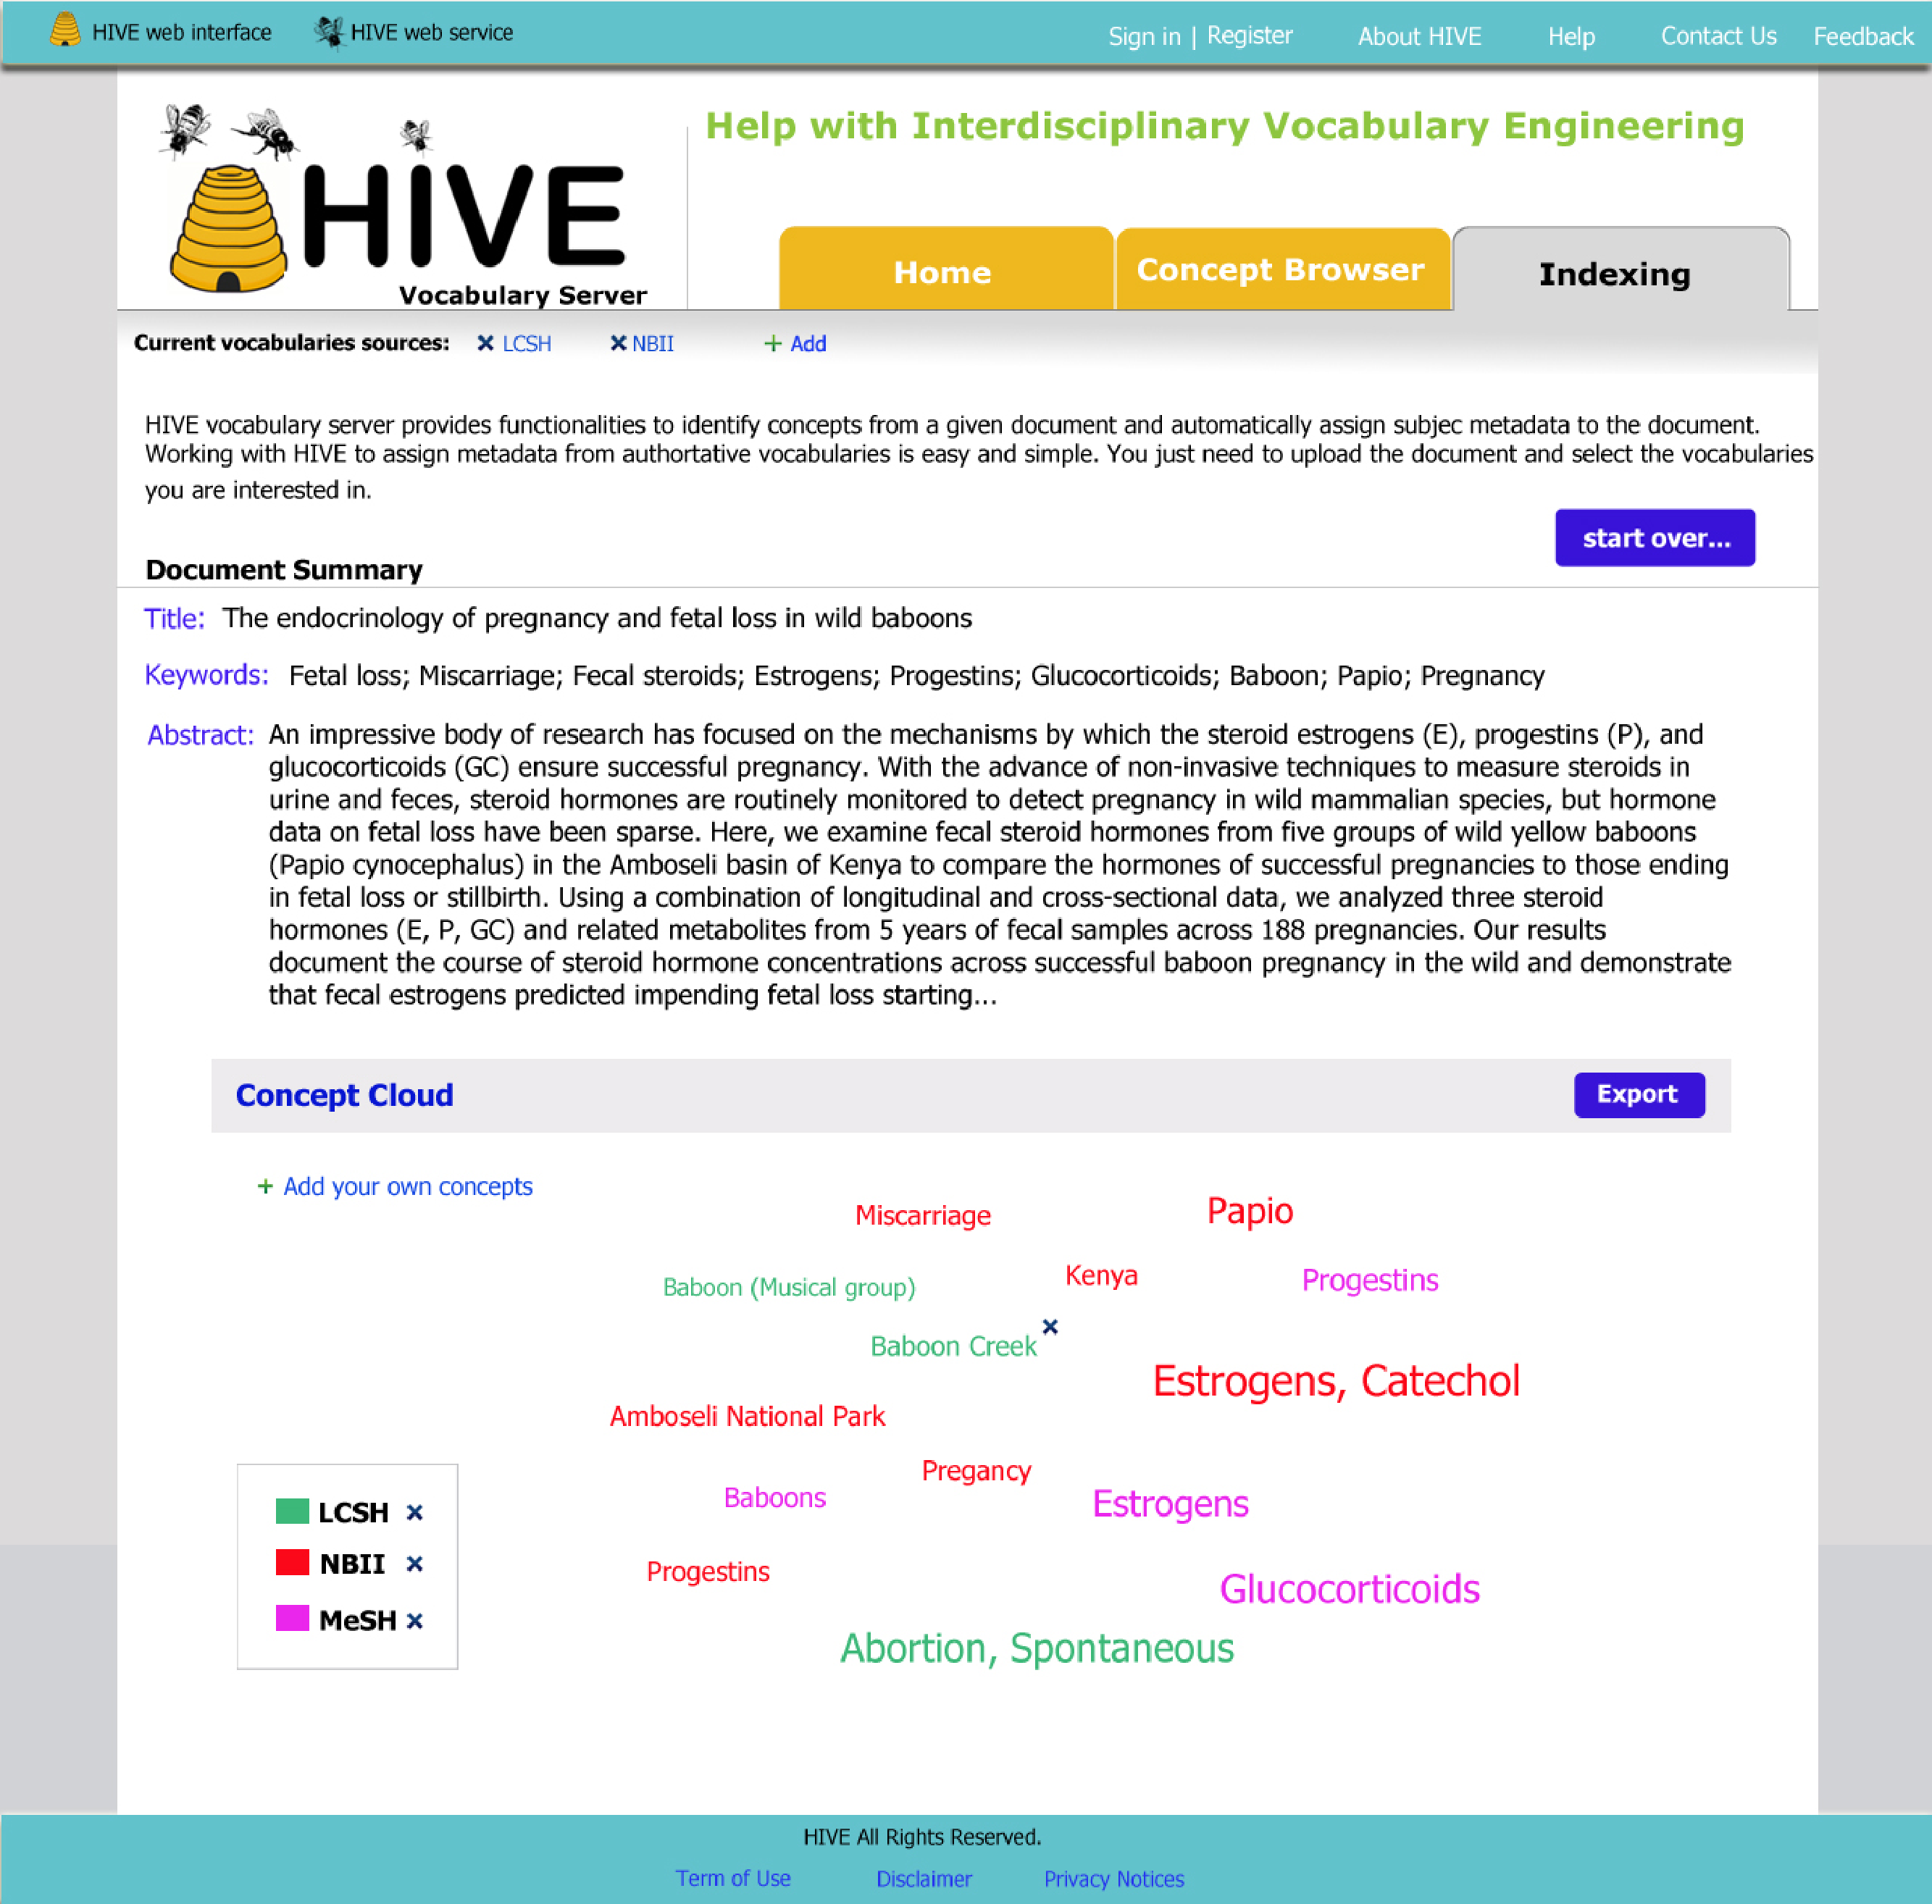
\includegraphics[width=400pt]{img/indexing.pdf}
\caption{Automatic Annotation tool}
\label{indexing}
\end{figure}

HIVE Concept Browser, showed in figure \ref{browser} is the most important component of HIVE Web UI. The HIVE Concept Browser also 
articulates the RIA paradigm applied in the design and implementation process.

\begin{figure}
\centering
\includegraphics[width=400pt]{img/browser.pdf}
\caption{Concept Browser}
\label{browser}
\end{figure}

The goal of HIVE Concept Browser is to allow users to browse and search concepts from heterogeneous 
vocabulary authorities such as Library of Congress Subject Headings and National Biological Information 
Infrastructure. The other important aspect of Concept Browser is to visualize the context of concept 
via showing the relations to help user better understand difficult concept as well as its usage. 
The functionalities of Concept Browser include:

\begin{itemize}
\item Allow user to traverse from different vocabularies.
\item Allow user to open and close a vocabulary.
\item Allow user to search concepts in multiple vocabularies, and filtering the concepts based on user 
selection.
\item Visualize the hierarchical structure of user selected vocabulary for browsing.
\item Visualize the context of concepts to help user better understand difficult concept.
\item Display the concept in SKOS metadata schema.
\end{itemize}

%\begin{figure}
%\centering
%\psfig{file=browser.pdf, height=2.7in, width=3.3in,}
%\caption{HIVE Concept Browser}
%\label{browser}
%\end{figure}

The design principles of the functionalities described above are based on RIA, and the implementation are 
powered by RIA technology, Google Web Tool Kit. Future work on HIVE Web UI will focus on the usability 
testing for the RIA feature to gain a constructive understanding of impact of RIA technologies on the 
usability of interactive web application.

\subsection{Linked data for concepts}

HIVE is a multi-vocabulary environment that allows access to concepts and vocabularies using a simple 
URL.  This idea was presented for LCSH, and 
we have generalized this approach for any vocabulary stored on a server.  HIVE implements the 
technological infrastructure to store millions of concepts from different vocabularies and make them 
available on the Web by a simple HTTP call based on RESTful paradigm.  Vocabularies can be imported in HIVE using SKOS/RDF format. 
As a result of this work, sharing concepts and vocabularies on the Web becomes easy and straightforward.

\section{Installing HIVE web}

The installation of the demo HIVE web is quite simple. as we have seen previously, HIVE web is based on GWT, so the installation is similar 
to other Java based applications.

HIVE web can be installed in application servers like tomcat or Resin. We have using Tomcat 6.0 for this document.

The main constraint is that HIVE web must be installed in the ROOt directory of your application server, because there is a bug in the GWT 
multipage module that has not been solved yet by the developers of this module (for the discussion about this you can read the thread in 
the GWT multipage web page http://claudiushauptmann.com/gwt-multipage/)

To run HIVE web in your application server you should follow the following steps:

\begin{itemize}
 \item Copy the content of the directory hiveweb in your HIVE distribution in the ROOT directory of your Tomcat installation.
 \item Go to the  ../WEB-INF/conf directory to configurate the configuration files.
\end{itemize}

There are to kind of configuration files in HIVE:

\begin{itemize}
 \item vocabularies: This is the general file for configuration. This file contains the information about the vocabularies that will 
be loaded when the application starts. So if we want load three vocabularies we will include its names in this file. You only can have 
one “vocabularies” file for each HIVE instance.
 \item $<vocabularyName>$.properties: These properties files include information about each vocabulary that can be loaded by the system. 
For example the file lcsh.properties will include information to load LCSH vocabulary in HIVE. This file not only have information about 
the vocabulary, but also have the paths to the different databases where the vocabulary is stored. As we said previously, HIVE have a 
double storage system, one based on Sesame RDF native databases and one based on Lucene. Lcsh.prperties will include the path in the 
file system to this databases. The format for these files in described in detail in \ref{configuration}.
\end{itemize}

\subsection{Memory problems}

If we need load a big amount of data in HIVE we will have to allocate more memory before start our Tomcat server.
To do that we will need to define a environment variable like this:

\begin{verbatim}
export CATALINA_OPTS="-Xmx1512m -XX:-UseGCOverheadLimit"
\end{verbatim}

with this variable we are allocating more memory for tomcat and we will avoid problems to load huge vocabularies on HIVE web.